\documentclass[a4paper]{article}
\usepackage[utf8]{inputenc}
\usepackage[spanish, es-tabla, es-noshorthands]{babel}
\usepackage[table,xcdraw]{xcolor}
\usepackage[a4paper, footnotesep = 1cm, width=20cm, top=2.5cm, height=25cm, textwidth=18cm, textheight=25cm]{geometry}
%\geometry{showframe}

\usepackage{tikz}
\usepackage{amsmath}
\usepackage{amsfonts}
\usepackage{amssymb}
\usepackage{float}
\usepackage{graphicx}
\usepackage{caption}
\usepackage{subcaption}
\usepackage{multicol}
\usepackage{multirow}
\setlength{\doublerulesep}{\arrayrulewidth}
\usepackage{booktabs}

\usepackage{hyperref}
\hypersetup{
    colorlinks=true,
    linkcolor=blue,
    filecolor=magenta,      
    urlcolor=blue,
    citecolor=blue,    
}

\newcommand{\quotes}[1]{``#1''}
\usepackage{array}
\newcolumntype{C}[1]{>{\centering\let\newline\\\arraybackslash\hspace{0pt}}m{#1}}
\usepackage[american]{circuitikz}
\usetikzlibrary{calc}
\usepackage{fancyhdr}
\usepackage{units} 
\usepackage{svg}

\graphicspath{{../Ejercicio-1/}{../Ejercicio-2/}{../Ejercicio-3/}{../Ejercicio-4/}{../Ejercicio-5/}}
%\svgpath{{../Ejercicio-1/}{../Ejercicio-2/}{../Ejercicio-3/}{../Ejercicio-4/}{../Ejercicio-5/}}

\pagestyle{fancy}
\fancyhf{}
\lhead{22.05 ASSD}
\rhead{Mechoulam, Lambertucci, Rodriguez, Londero}
\rfoot{Página \thepage}

\begin{document}
Para este ejercicio se implemento el decodificador de direcciones con un integrado 74LS138 y lógica combinacional.
Valiendonos de que dado a que únicamente se utilizaran estos 4 periféricos es posible asignar cantidades de memoria por demás a los periféricos.
quedando de la siguiente manera la tabla de direcciones.
\begin{table}[H]
\centering
\begin{tabular}{|c|c|c|c|}
\hline
Adress & Dispositivo & Binario Comienzo & Binario Fin \\ \hline
C000 & ROM16K & 1100000000000000 & 1111111111111111 \\ \hline
A800 & Entrada 8 Bits & 1010100000000000 & 1011111111111111 \\ \hline
A000 & Salida 8 Bits & 1010000000000000 & 1010011111111111 \\ \hline
2000 & RAM4K & 0010000000000000 & 0010111111111111 \\ \hline
\end{tabular}
\end{table}
Basta con conectar los siguientes bits con el decoder
\begin{align}
a_{14} \implies C\\
a_{15} \implies B\\
a_{11} \implies A
\end{align}
así también conectar las salidas $Y_0$ $Y_1$  con una compuerta or, al igual que las $Y_6$ $Y_7$ con otra.
quedando definidos los chip select de la siguiente manera.

\begin{figure}[H]
  \centering
  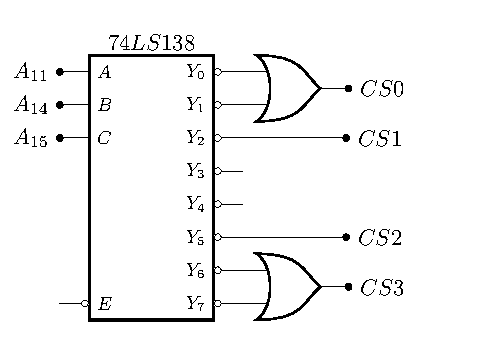
\includegraphics[width=.6\textwidth, page = 1]{ImagenesEjercicio2/Circuits.pdf}
  \caption{Diagrama en bloques}.
  \label{fig:fotofea}
\end{figure}

\end{document}